\section{Methodology}
\label{sec:methodology}

In this work, we adapt a pre-trained video generation model for \textbf{video reshooting}: the task of modifying the camera trajectory of an existing video while preserving its content and visual style. We first define the task, then describe our novel self-supervised data pipeline, and finally detail the architectural adaptations and training augmentations required to implement our approach.


\begin{figure*}
    \centering
    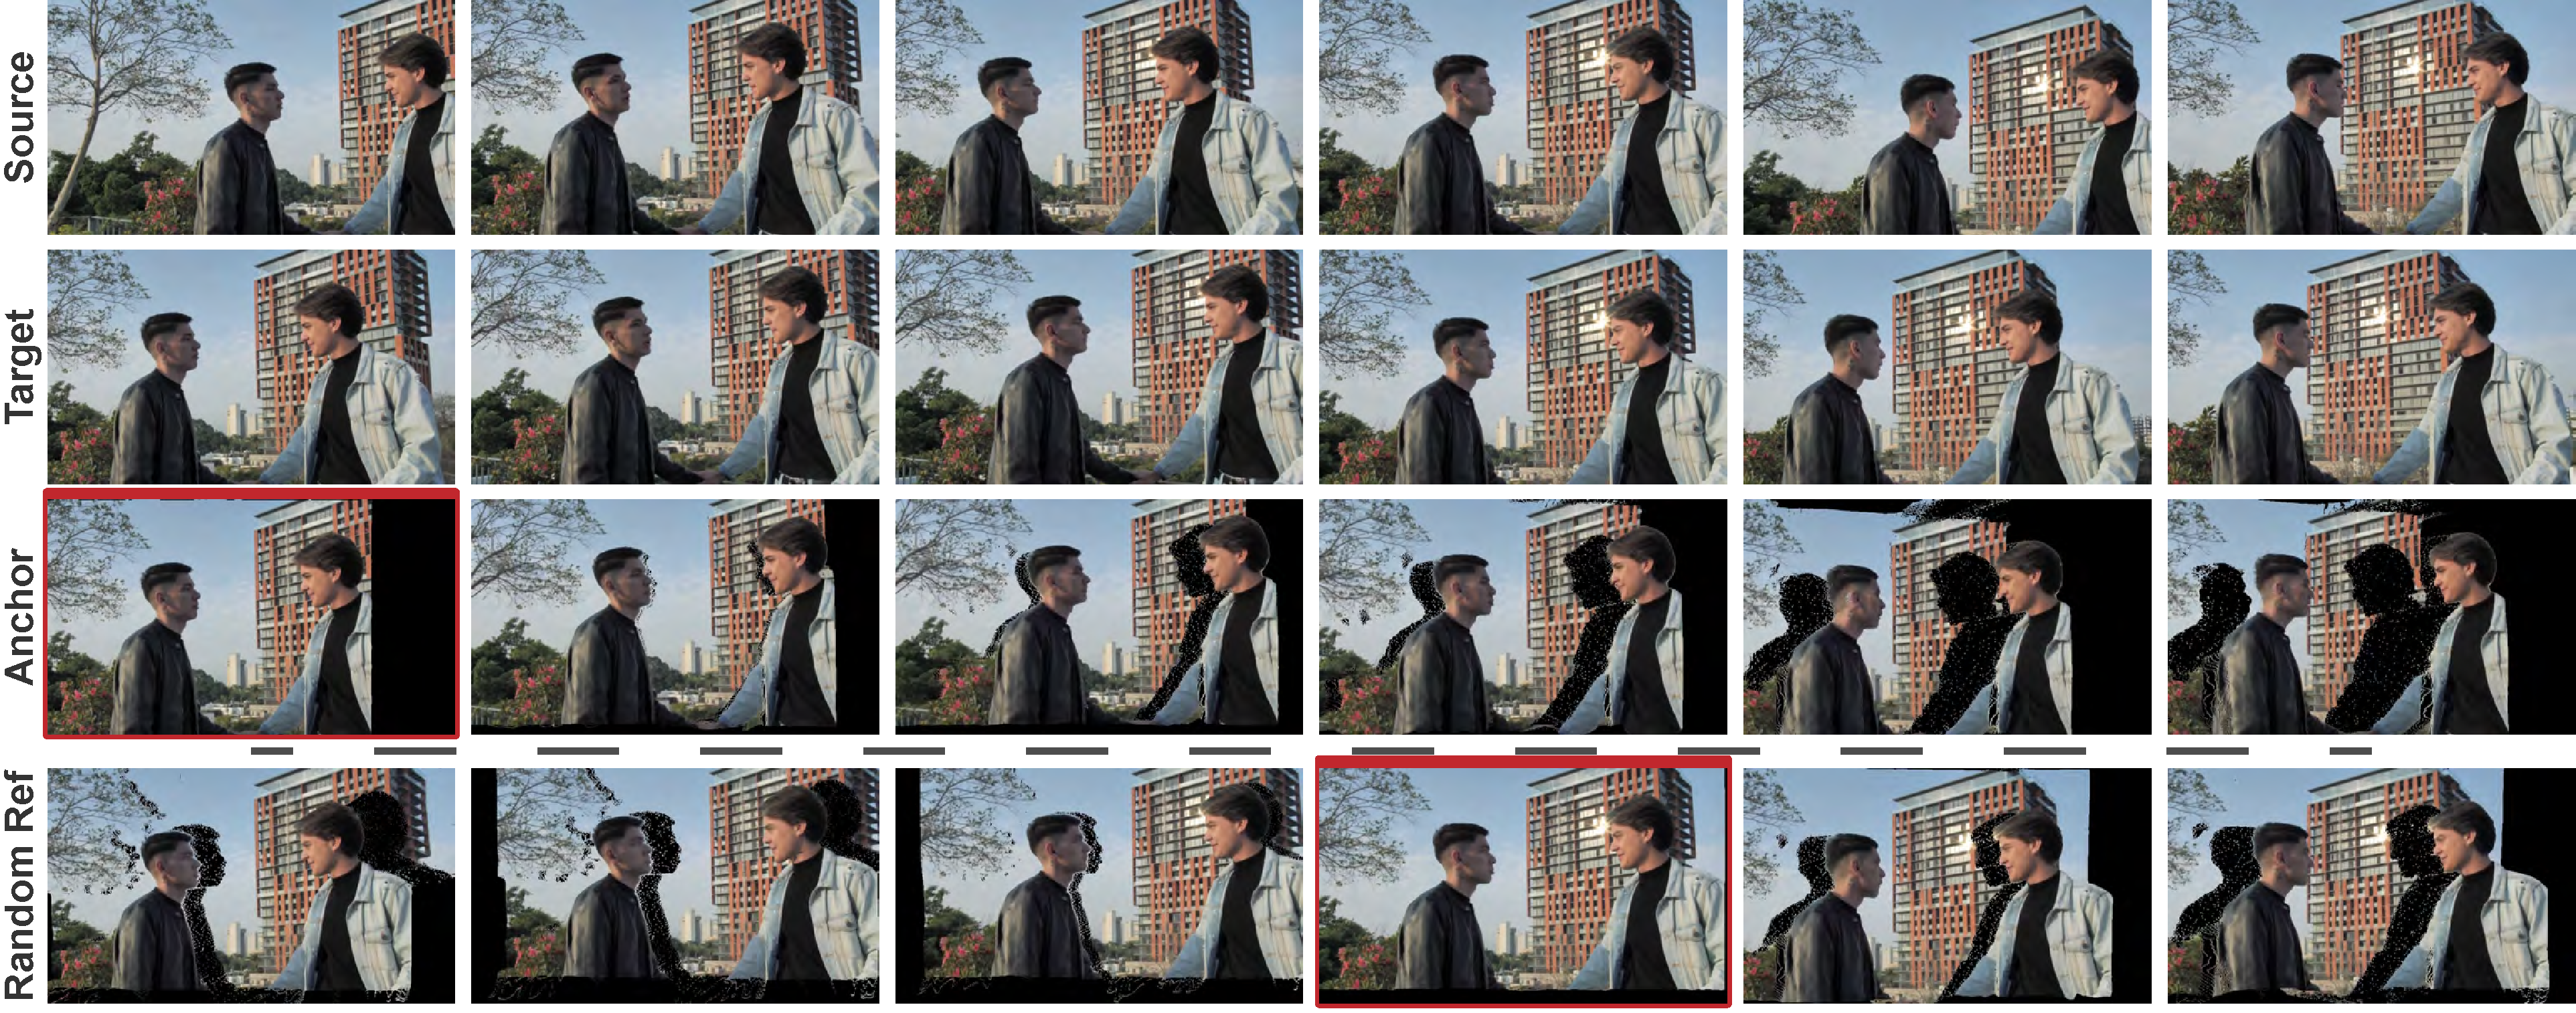
\includegraphics[width=\linewidth]{figures/video_triplets.pdf}
    \vspace{-0.25in}
    \caption{
        \textbf{Our Pseudo Multi-View Triplet and Training Augmentations.}
        The \textbf{top three rows} illustrate our core training triplet: the \textit{Source Video} ($V_s$), the \textit{Target Video} ($V_t$), and the synthetically generated \textit{Anchor Video} ($V_a$). By default, $V_a$ is created by forward-warping a reference frame from $V_s$ to align with the $V_t$ trajectory. This process can incorporate augmentations such as 3D-aware noise injection (into the $V_s$ reference frame before warping) and flexible reference frame selection, simulating inference-time artifacts and promoting robustness (see Section~\ref{sec:technical_augmentations}).
        The \textbf{bottom row} shows an example of our Flexible Anchor Reference Frame Warping augmentation, varying the reference frame for robustness. More details are in the Supplementary Material.
    }
    \label{fig:triplets}
    \vspace{-0.2in}
\end{figure*}

The video reshooting task requires synthesizing a high-fidelity \textit{target video}, $V_{t}$, based on a new, desired camera path. At inference time, our model is conditioned on two primary inputs: the \textit{source video} ($V_{s}$), which is the original, high-quality monocular video serving as the texture and content reference; and the \textit{anchor video} ($V_{a}$), which defines the target camera motion. This anchor video is typically pre-rendered from a 3D representation of the original scene.

Following recent approaches~\cite{yu2025trajectorycrafter,ex4d,jeong2025reangle,bai2024syncammaster,wang2025epic}, we utilize an anchor video as a primary conditioning signal. This choice is crucial for two main reasons:
\begin{description}[noitemsep, topsep=0pt, partopsep=0pt, leftmargin=0pt, style=unboxed, font=\normalfont\bfseries]
    \item [Intuitive Visual Guidance:] An anchor video offers a dense, intuitive visual representation of the target camera trajectory, empirically more effective for guiding generative models than explicit camera poses.
    \item [Self-Supervised Training Necessity:] It is essential for our novel self-supervised training strategy (detailed in Section~\ref{sec:self_supervision}). Our method generates pseudo-views from 2D crops without modifying underlying 3D camera parameters, making relative camera poses non-viable. The anchor video instead provides the concrete spatiotemporal target needed for our pseudo multi-view training pairs.
\end{description}

This anchor video ($V_a$) is inherently imperfect, suffering from artifacts like holes and inaccuracies from depth/pose estimation. While unsuitable for direct viewing, it is crucial for defining the target trajectory. The model's core task is to generate $V_{t}$ that faithfully follows $V_{a}$'s motion, replacing its distorted content with clean, temporally consistent texture from $V_{s}$. Training this two-stream model ideally requires large-scale triplets $(V_{s}, V_{a}, V_{t})$ with pristine $V_t$ ground-truth, which is logistically intractable. We address this with our novel self-supervised approach, generating these triplets from monocular videos alone, as described next.

\subsection{Self-Supervision from Monocular Video}
\label{sec:self_supervision}

To address the challenges of data acquisition, we introduce a novel self-supervised strategy that synthesizes the required $(V_s, V_a, V_t)$ training triplets solely from abundant monocular videos.

\subsubsection{Pseudo-View Triplet Generation}
\label{sec:pseudo_view_triplet}

From a single input video $V$, we first employ a smooth video cropper to generate two distinct clips. These clips, which will form our \textit{source video} ($V_s$) and \textit{target video} ($V_t$) for the training triplet, each follow independent \textit{smooth random-walk trajectories} that emulate dynamic camera motion, as shown in Figure~\ref{fig:teaser}. Each trajectory is generated by sampling an adaptive number of random control points within the frame boundaries, with the overall motion magnitude governed by a tunable scale parameter. A \textit{natural cubic spline} is then fitted through these control points to produce a continuous and smooth crop trajectory.

\begin{figure*}
    \centering
    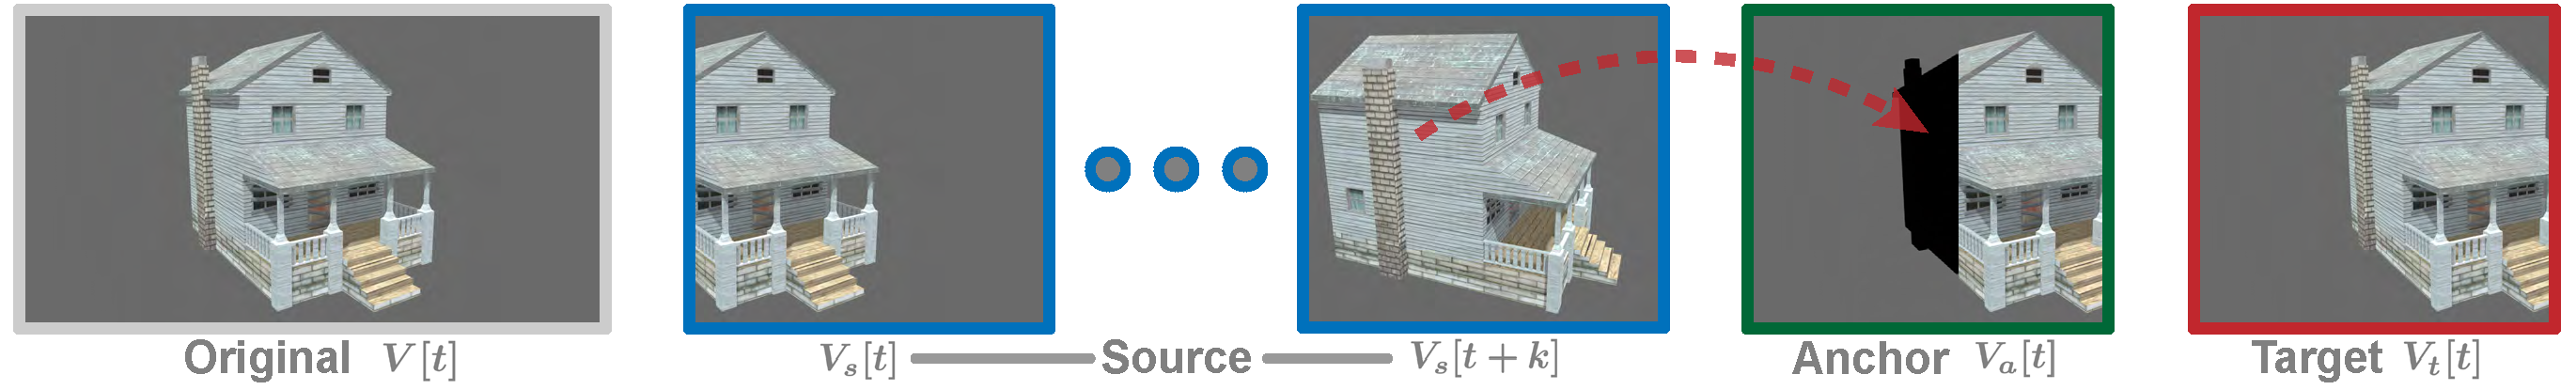
\includegraphics[width=0.8\linewidth]{figures/impl_reprojection.pdf}
    \vspace{-0.1in}
    \caption{
    \textbf{Implicit 3D Reasoning in our Self-Supervised Setup.}
    Our training method forces the model to learn 3D structure from 2D data.
    To reconstruct the \textit{Target} $V_t$ at frame $t$, the model is given the disoccluded (holed) \textit{Anchor} $V_a[t]$.
    The corresponding \textit{Source} frame $V_s[t]$ may not contain the missing texture (e.g., the side of the building).
    The model is forced to find this texture in a different source frame, $V_s[t+k]$, where it is visible due to $V_s$'s independent camera motion.
    This operation of sourcing and "stitching" content across different times and pseudo-viewpoints compels the model to learn an implicit 3D understanding of the scene.
    % \todo{ADD ATTRIBUTION IN FINAL VERSION}
    }
    \label{fig:implicit_3d}
    \vspace{-0.2in}
\end{figure*}

We sample two trajectories using different random seeds, resulting in clips $(V_{s}, V_{t})$ that observe different regions of the same video, effectively mimicking time-synchronized distinct moving cameras. Importantly, the original video $V$ may already exhibit its own inherent camera motion; our method naturally inherits and compounds this motion, capturing complex patterns such as orbits, pans, and zooms from in-the-wild footage.

We designate the two clips as the \textit{Target Video ($V_{t}$)}, the clip to be reconstructed, and the \textit{Source Video ($V_{s}$)}, the high-fidelity texture reference. Based on both clips, we then synthetically generate the \textit{Anchor Video ($V_{a}$)} to complete the training triplet ($V_{s}, V_{a}, V_{t}$), as described next.

We generate $V_{a}$ by warping the first frame of the source video ($V_{s}[0]$) to align with the target video's trajectory ($V_{t}$). This warping process, illustrated in Figure~\ref{fig:triplets}, is guided by an offset-aware flow field that combines two components: (1) a dense tracking field (capturing 2D pixel motion) and (2) an \textit{crop offset flow} (capturing the change in pseudo-viewpoint). To obtain the dense tracking field, we use AllTracker~\cite{4d_recon_harley2025alltracker} on the original video $V$ \textit{before} cropping. We chose this state-of-the-art tracking method as it is more effective than simple two-frame optical flow for computing correspondences over long temporal distances, as it leverages all intermediate frames. This combined flow is then used to forward-warp $V_{s}[0]$ over time using softmax splatting~\cite{softmax_splatting}:
\begin{equation}
V_{a}[t] = \text{SoftSplat}(V_s[0], F_{\text{comb}}(t)),
\label{eq:anchor_warping}
\end{equation}
where $V_a[t]$ is the $t$-th frame of the anchor video, $\text{SoftSplat}$ is the forward warping operator, and $F_{\text{comb}}(t)$ is our combined offset-aware flow field that maps pixels from $V_s[0]$ to the $t$-th frame of the target's coordinate system. The use of forward warping is a deliberate choice, as it effectively simulates the artifacts, occlusions, and dis-occlusions characteristic of the point-cloud-based anchor videos we use at inference.

\subsubsection{Implicit 3D-Aware Learning}
\label{sec:implicit_3d_learning}

This training setup directly forces the model to learn its inference-time task. It must learn to reconstruct the high-quality, dynamic $V_{t}$ by:

\begin{description}[noitemsep, topsep=0pt, partopsep=0pt, leftmargin=0pt, style=unboxed, font=\normalfont\bfseries]
    \item[Ignoring Anchor Artifacts] The model learns to treat $V_{a}$ as a geometric guide, not a texture source.
    \item[Spatial Content Sourcing] The model is forced to find the correct, high-fidelity textures from $V_{s}$. Because $V_{s}$ and $V_{t}$ are not spatially aligned, the model must use its attention mechanism to find content in different spatial regions of the source.
    \item[Implicit 3D Reasoning] This setup compels the model to reason about 3D structure. As illustrated in Figure~\ref{fig:implicit_3d}, consider the task of reconstructing frame $t$ of the target video, $V_t$. This frame may contain a disoccluded region (e.g., the side of a building) that is not visible in the corresponding source frame $V_s[t]$. However, because the source video $V_s$ has its own independent camera motion, that same side of the building might be visible in a different frame, $V_s[t+k]$. The model is therefore forced to learn to find and source this non-aligned information, effectively "stitching" a view from $V_s[t+k]$ into the disoccluded hole at frame $t$. This operation of finding and re-projecting texture across different viewpoints and times is a form of implicit 3D reasoning.
    \item[Generative In-painting] For any regions that are not visible in \textit{any} $V_{s}$ frame, the model learns to leverage the generative priors of the base model to plausibly in-paint (or "hallucinate") the missing details.
\end{description}




This self-supervised strategy has several key advantages over synthetic or 3D-annotated approaches, primarily in its simplicity and scalability. Our entire data pipeline relies only on a robust 2D dense tracker. This is a significant advantage, as 2D tracking methods are generally more mature and accurate than 3D annotation techniques. This simplicity means our pipeline is domain-agnostic and can be applied to virtually any monocular video. As a result, we can train on a vast and diverse corpus that includes \textit{photorealistic footage, animation, gaming content, and even videos generated by other Gen-AI models}. This exposes our model to a rich variety of both complex visual phenomena (e.g., water splashing, lens flares) and diverse camera motions (e.g., shaky handheld, professional dolly zooms), all without the domain limitations of synthetic generation.

It is important to note that our training objective does not directly optimize for 3D reconstruction. Rather, the model is compelled to \textit{implicitly learn} 3D reasoning as a necessary sub-task. In order to successfully reconstruct the target video $V_t$ by sourcing content from $V_s$ and following the geometry of $V_a$, the model must learn to handle occlusions and re-project textures across distinct viewpoints and times from the source video to reconstruct the target video, guided by the anchor video. Therefore, 3D re-rendering emerges as a subset of the capabilities our model learns to solve this complex 2D-based task. This full methodology, combining a domain-agnostic pipeline with a generative diffusion base, produces a model that can also plausibly in-paint, hallucinate realistic textures, and robustly handle diverse video styles in a way that pure 3D reconstruction methods cannot.

\subsection{Model Architecture and Conditioning}
\label{sec:architecture}

\begin{figure*}
    \centering
    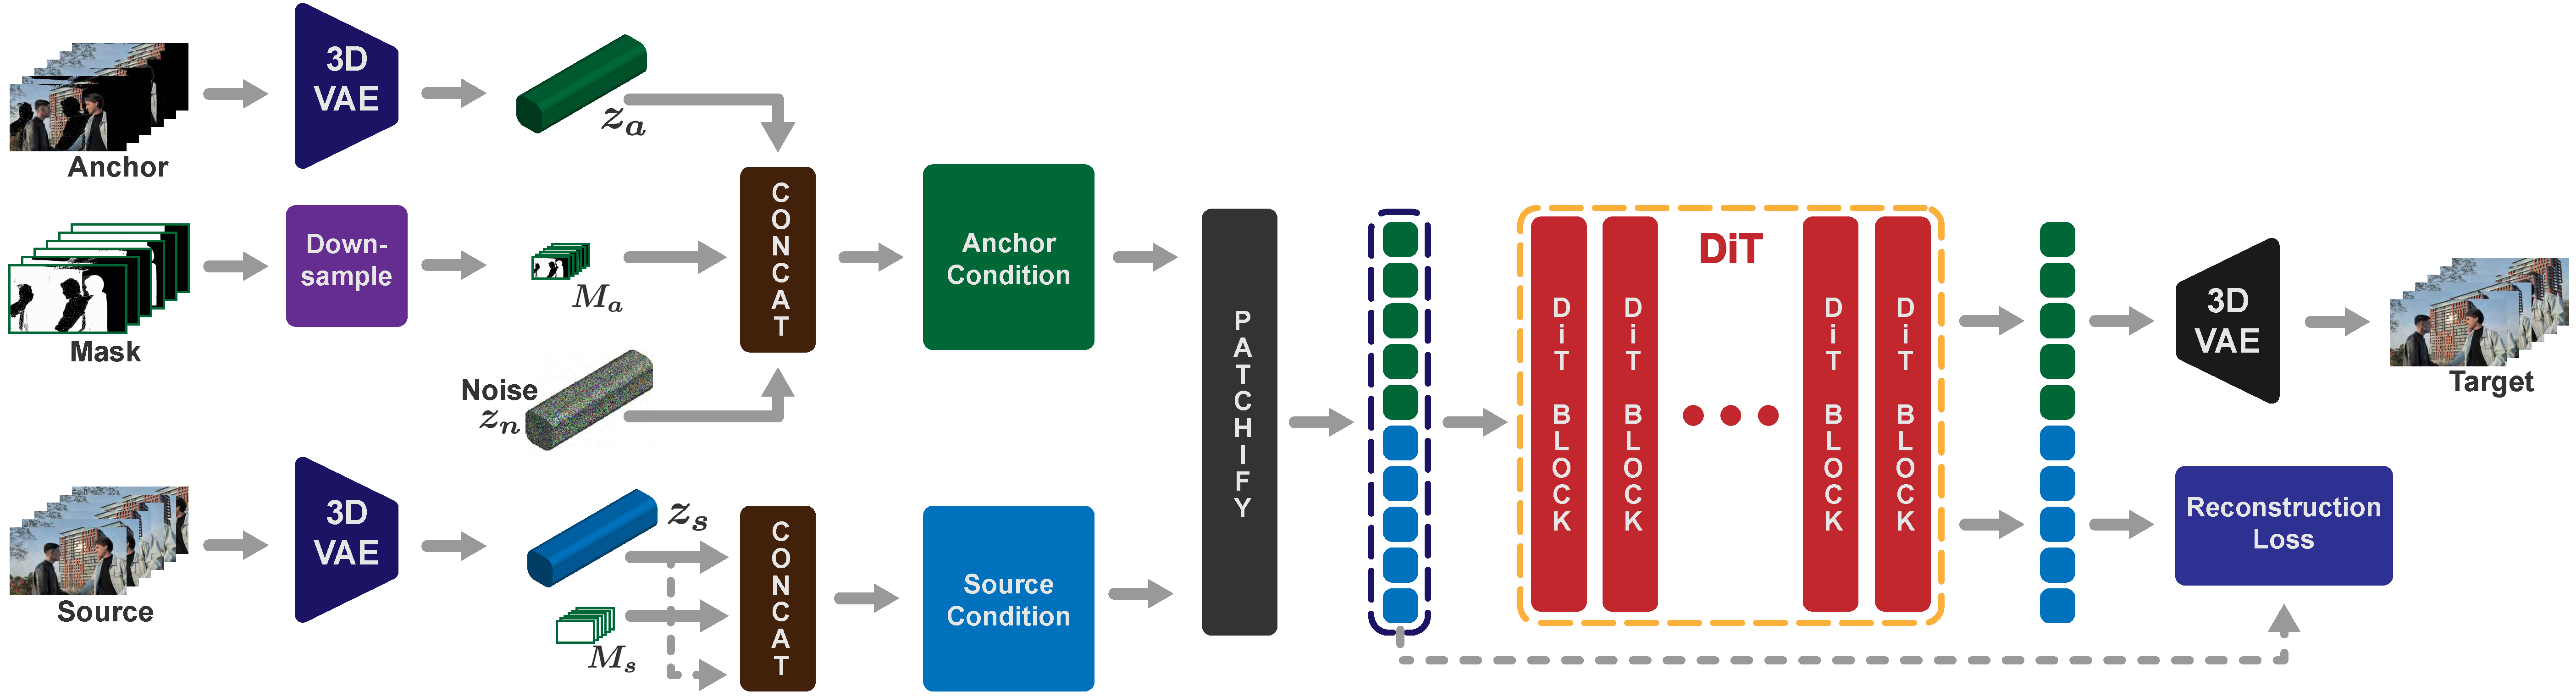
\includegraphics[width=0.8\linewidth]{figures/overview.pdf}
    \vspace{-0.13in}
    \caption{\textbf{Overview of our Conditioning Architecture.} Our model adapts a pre-trained DiT-based I2V model~\cite{wan21}. \textbf{(1) VAE Encoding:} The Anchor video ($V_a$) and Source video ($V_s$) are independently encoded into latents by the VAE ($z_a, z_s$). \textbf{(2) Conditioning Setup:} The Anchor latent ($z_a$) is combined with a noise latent ($z_{n}$) and its corresponding mask ($M_a$). The Source latent ($z_s$) is duplicated (replacing $z_{n}$) and combined with an all-ones mask ($M_s$). \textbf{(3) DiT Processing:} The two conditioned streams are temporally concatenated and fed into the DiT blocks. \textbf{(4) Source Token Management \& Denoising:} After each denoising step, the output tokens corresponding to the Source are subjected to an auxiliary reconstruction loss (ensuring content retention).}
    \label{fig:overview}
    \vspace{-0.2in}
\end{figure*}

Having established our self-supervised training data (Section~\ref{sec:self_supervision}), we now detail the architectural adaptations required to finetune a pre-trained video diffusion model for our task, as illustrated in Figure~\ref{fig:overview}.

\subsubsection{Video Diffusion Models and DiT Conditioning}
\label{sec:arch_background}

Our approach adapts a Diffusion Transformer (DiT) based video model, specifically the WAN 2.2 I2V architecture~\cite{wan21}. DiTs utilize a Transformer architecture for denoising latents, operating as Latent Diffusion Models (LDMs). In essence, the base model is trained to predict the denoised latent from a noisy input, effectively learning to reverse the diffusion process to generate high-quality video frames.


Conditional signals in DiT architectures can be integrated via: (1) channel concatenation with the noisy latent; (2) dedicated cross-attention layers; or (3) introduction as supplementary tokens processed by the full self-attention mechanism~\cite{bai2025recammaster, peebles2023scalable}. The chosen mechanism is critical for temporal modeling and the application of Rotary Positional Embeddings (RoPE), which encode relative spatiotemporal positional information within transformer blocks, enabling precise understanding of frame order and distance~\cite{bai2025recammaster, su2024roformer}. For our specific adaptations, we leverage a token-based conditioning approach as detailed in the following subsections.

\subsubsection{Source-Anchor Fusion with Offset RoPE}
\label{sec:offset_rope}

Our model leverages two primary conditions: an anchor video ($V_a$) for geometric guidance and a source video ($V_s$) for high-fidelity texture. Instead of using separate cross-attention for $V_s$, which often proves ineffective for this task as observed in~\cite{bai2025recammaster}, we process both $V_s$ and $V_a$ as tokens within the model's main self-attention mechanism (Figure~\ref{fig:overview}).

Both $V_a$ and $V_s$ are independently encoded into latents ($z_a, z_s$) by the pre-trained VAE. The Anchor condition combines $z_a$ with a noise latent ($z_n$) and its downsampled binary mask ($M_a$), indicating regions for generation. The Source condition uses $z_s$ with an all-ones mask ($M_s$), ensuring all content is leveraged. These two prepared conditional streams are then temporally concatenated and fed into the DiT blocks.

Within each DiT block, 3D Rotary Positional Embeddings (RoPE) are applied. To enable robust, flexible-length video generation and overcome fixed-length constraints of naive RoPE~\cite{bai2025recammaster}, we implement an \textit{Offset RoPE}. A large, fixed offset is applied only to the temporal positional embeddings of the $V_s$ tokens. This effectively decouples the source condition's perceived position from the target's, allowing for flexible sequence lengths at inference without retraining.

A crucial aspect is managing source tokens after each denoising step. While their output tokens are discarded (as they don't directly form $V_t$), an auxiliary reconstruction loss is applied during training between the output source tokens and their original clean VAE latents ($z_s$). This encourages the source pathway to preserve content from $V_s$, supporting more effective texture sourcing. Only the denoised anchor tokens contribute to the primary diffusion loss or subsequent denoising steps. Further implementation details are in the Supplementary Material.


\begin{table*}[t]
\label{table-main-comparison}
	\begin{center}
\vspace{-0.30cm}
		\caption{Quantitative comparison with SOTA methods on VBench, temporal consistency, camera accuracy, and view synchronization.}
\vspace{-0.30cm}
		\label{tab_merged_eval}
		\setlength\tabcolsep{3.2pt} % Keep small for fitting
 	\centering
 	\resizebox{\textwidth}{!}{ % Use \textwidth to fit the wide table
		\begin{tabular}{lcccccc|c|cc|ccc}
			\toprule
			\multirow{2}{*}{Method}
            & \multicolumn{6}{c|}{VBench Quality}
            & \multicolumn{1}{c|}{Temporal Consistency}
            & \multicolumn{2}{c|}{Camera Accuracy}
            & \multicolumn{3}{c}{View Synchronization} \\
     	\cmidrule(lr){2-7}
     	\cmidrule(lr){8-8}
     	\cmidrule(lr){9-10}
     	\cmidrule(lr){11-13}
            & \makecell[c]{Aesthetic $\uparrow$} & \makecell[c]{Imaging $\uparrow$} & \makecell[c]{Flickering $\uparrow$} & \makecell[c]{Smoothness $\uparrow$} & \makecell[c]{Subject $\uparrow$} & \makecell[c]{Background $\uparrow$}
			& CLIP-F $\uparrow$
			& RotErr $\downarrow$
			& TransErr $\downarrow$
			& Mat. Pix $\uparrow$
			& FVD-V $\downarrow$
			& CLIP-V $\uparrow$ \\
		\midrule

	\trajectorycrafter{} (49 frames) & 52.69 & \textbf{59.67} & 96.97 & 99.03 & 93.78 & 95.13 & 98.80 &  \textbf{2.26} & 3.03 & 1851.80 & 582.56 & 92.40 \\
	\textbf{Ours} (49 frames) & \textbf{52.72} & 57.81 & \textbf{97.43} & \textbf{99.24} & \textbf{95.09} & \textbf{95.62} & \textbf{99.01} & 2.61 & \textbf{2.73} & \textbf{2737.65} & \textbf{488.22} & \textbf{94.96} \\
    \midrule
    \midrule
	\recammaster{} & 48.71 & 52.61 & \textbf{97.57} & \textbf{99.26} & 88.57 & 90.65 & 98.49 & 11.29 & 19.59 & 1314.00 & 732.52 & 88.91 \\
	\exfd{} & 49.72 & 55.76 & 97.46 & 99.08 & 91.51 & 94.78 & 98.94 & 3.94 & \textbf{4.21} & 2188.98 & 685.63 & 89.77 \\
	% \textbf{Ours} & 53.05 & 58.39 & 97.42 & 99.20 & 93.43 & 95.11 & 99.04 & 3.27 & 4.92 & 2636.07 & 595.39 & 92.94 \\
    \midrule
    \textbf{Ours w/o Source Video} & \textbf{53.97} & \textbf{58.92} & 97.13 & 98.99 & 93.12 & 95.03 & 98.95 & 4.82 & 11.65 & 226.01 & 662.09 & 89.97 \\
    \textbf{Ours} & 52.85 & 58.64 & 97.37 & 99.21 & \textbf{93.43} & \textbf{95.24} & \textbf{99.03} & \textbf{2.76} & 4.23 & \textbf{2720.83} & \textbf{586.24} & \textbf{93.16} \\
\bottomrule
		\end{tabular}
 	}
	\end{center}

    \vspace{-0.33in}
\end{table*}




% \begin{table*}[t]
% \label{table-main-comparison}
% 	\begin{center}
% \vspace{-0.30cm}
% 		\caption{Quantitative comparison with SOTA methods on VBench, temporal consistency, camera accuracy, and view synchronization.}
% \vspace{-0.30cm}
% 		\label{tab_merged_eval}
% 		\setlength\tabcolsep{3.2pt} % Keep small for fitting
%  	\centering
%  	\resizebox{\textwidth}{!}{ % Use \textwidth to fit the wide table
% 		\begin{tabular}{lcccccc|c|cc|ccc}
% 			\toprule
% 			\multirow{2}{*}{Method}
%             & \multicolumn{6}{c|}{VBench Quality}
%             & \multicolumn{1}{c|}{Temporal Consistency}
%             & \multicolumn{2}{c|}{Camera Accuracy}
%             & \multicolumn{3}{c}{View Synchronization} \\
%      	\cmidrule(lr){2-7}
%      	\cmidrule(lr){8-8}
%      	\cmidrule(lr){9-10}
%      	\cmidrule(lr){11-13}
%             & \makecell[c]{Aesthetic $\uparrow$} & \makecell[c]{Imaging $\uparrow$} & \makecell[c]{Flickering $\uparrow$} & \makecell[c]{Smoothness $\uparrow$} & \makecell[c]{Subject $\uparrow$} & \makecell[c]{Background $\uparrow$}
% 			& CLIP-F $\uparrow$
% 			& RotErr $\downarrow$
% 			& TransErr $\downarrow$
% 			& Mat. Pix $\uparrow$
% 			& FVD-V $\downarrow$
% 			& CLIP-V $\uparrow$ \\
% 		\midrule

% 	\trajectorycrafter{} (49 frames) & 52.69 & \textbf{59.67} & 96.97 & 99.03 & 93.78 & 95.13 & 98.80 & \textbf{2.26} & 3.03 & 1851.80 & 582.56 & 92.40 \\
% 	\textbf{Ours} (49 frames) & \textbf{52.72} & 57.81 & \textbf{97.43} & 99.24 & 95.09 & 95.62 & 99.01 & 2.61 & 2.73 & 2737.65 & 488.22 & 94.96 \\
%     \midrule
% 	\recammaster{} & 48.71 & 52.61 & \textbf{97.57} & \textbf{99.26} & 88.57 & 90.65 & 98.49 & 11.29 & 19.59 & 1314.00 & 732.52 & 88.91 \\
% 	\exfd{} & 49.72 & 55.76 & 97.46 & 99.08 & 91.51 & 94.78 & 98.94 & 3.94 & \textbf{4.21} & 2188.98 & 685.63 & 89.77 \\
% 	% \textbf{Ours} & 53.05 & 58.39 & 97.42 & 99.20 & \textbf{93.43} & 95.11 & 99.04 & 3.27 & 4.92 & 2636.07 & 595.39 & 92.94 \\
%     \midrule
%     \textbf{Ours w/o Source Video} & \textbf{53.97} & \textbf{58.92} & 97.13 & 98.99 & 93.12 & 95.03 & 98.95 & 4.82 & 11.65 & 226.01 & 662.09 & 89.97 \\
%     \textbf{Ours} & 52.85 & 58.64 & 97.37 & 99.21 & 93.43 & 95.24 & 99.03 & 2.76 & 4.23 & \textbf{2720.83} & \textbf{586.24} & \textbf{93.16} \\
% \bottomrule
% 		\end{tabular}
%  	}
% 	\end{center}

%     \vspace{-0.33in}
% \end{table*}




\subsubsection{Technical Augmentations for Robust Training}
\label{sec:technical_augmentations}

Beyond our core architecture, we integrate several technical augmentations to enhance model robustness and generation quality. Detailed configurations are provided in the Supplementary Material.

\begin{description}[noitemsep, topsep=0pt, partopsep=0pt, leftmargin=0em, style=unboxed, font=\normalfont\bfseries]
    \item[Source Token Reconstruction Loss] Auxiliary loss applied to ensure content retention from the source video.
    \item[Adaptive Anchor Mask Background Treatment] We use a high-contrast background (e.g., fluorescent pink) in masked-out regions of the anchor video to improve generation quality, especially in dark scenes.
    \item[Flexible Anchor Reference Frame Warping] Randomly selecting the reference frame for anchor warping increases robustness to diverse tracking conditions and prevents bias towards early frames.
    \item[3D-Aware Noise] Gaussian noise is applied to anchor's reference frame before warping, suppressing texture copying from the anchor while preserving its geometric guidance.
\end{description}

The detailed implementation of these augmentations is provided in Supplementary.


\begin{figure}
    \centering
    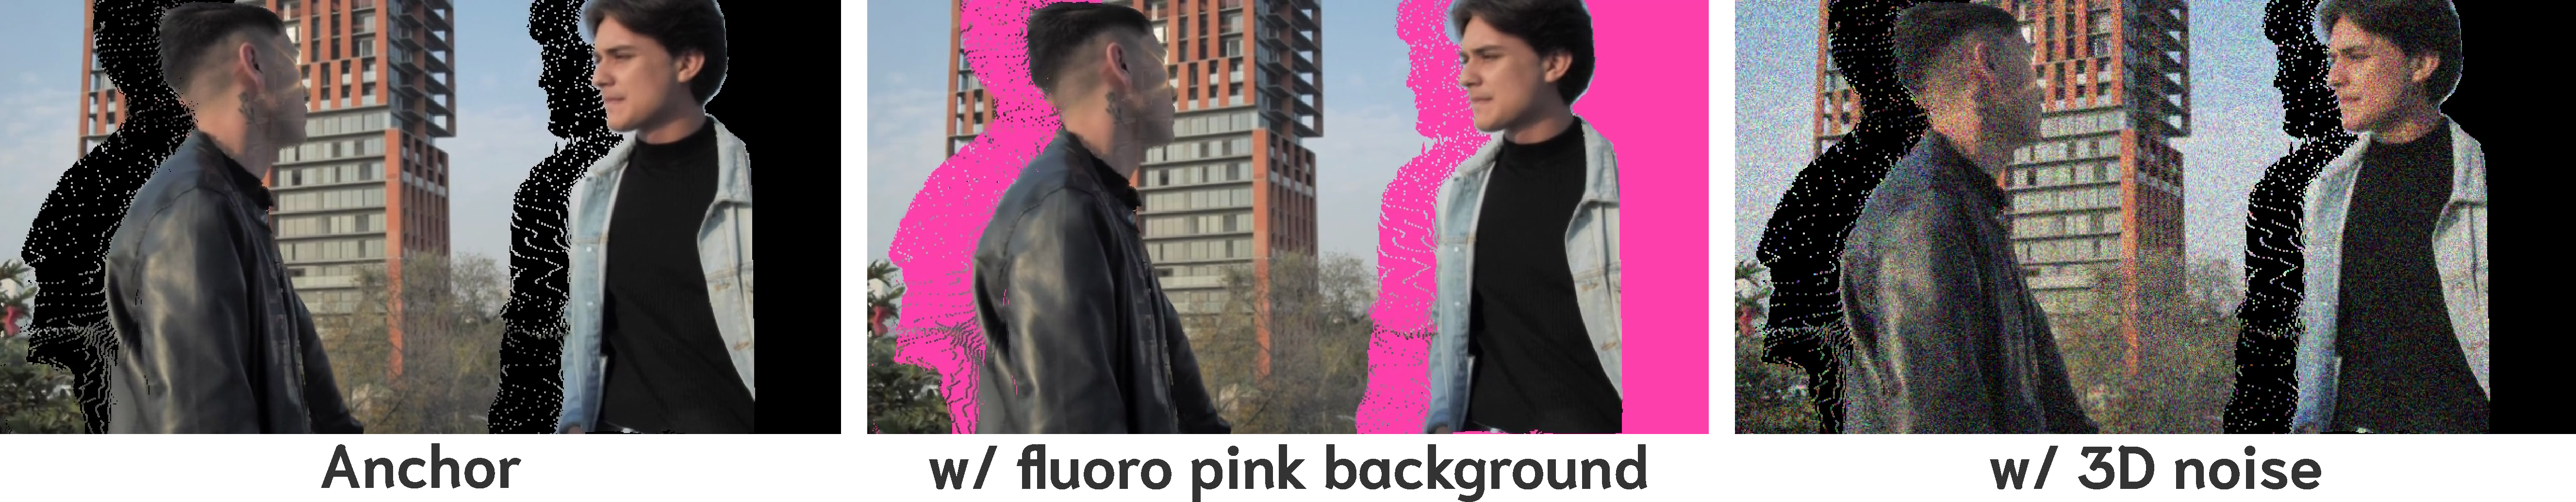
\includegraphics[width=\linewidth]{figures/ablations_input.pdf}
    \vspace{-0.25in}
    \caption{\textbf{Visualizing Anchor Video Augmentations.} This figure demonstrates key augmentations applied during Anchor Video ($V_a$) generation, shown on a single frame. From left to right: the default anchor with a black masked background; an anchor using a fluorescent pink background for masked regions; and an anchor with 3D-aware noise coherently injected into its reference frame. These techniques improve model robustness and help mitigate artifacts in challenging scenes (Section~\ref{sec:technical_augmentations}).}
    \label{fig:ablations_input}
    \vspace{-0.2in}
\end{figure}